\documentclass[conference]{IEEEtran}
\IEEEoverridecommandlockouts

\usepackage{cite}
\usepackage{amsmath,amssymb,amsfonts}
\usepackage{graphicx}
\usepackage{textcomp}
\usepackage{xcolor}
\usepackage{booktabs}
\usepackage{url}
\usepackage{comment}


\graphicspath{{Figures/}}

\def\BibTeX{{\rm B\kern-.05em{\sc i\kern-.025em b}\kern-.08em
    T\kern-.1667em\lower.7ex\hbox{E}\kern-.125emX}}

\begin{document}

\title{Network-Oriented Evaluation of Semantic XR Video Transmission under Frame-Level Update Loss}

\author{
\IEEEauthorblockN{Ziquan Lin, Francesc Wilhelmi, and Boris Bellalta}
\IEEEauthorblockA{\textit{Department of Engineering}\\
\textit{Universitat Pompeu Fabra}\\
Barcelona, Spain}
}

\maketitle

\begin{abstract}
Extended reality (XR) video transmission requires high visual quality under tight bandwidth and latency constraints. This paper studies an AI-aided semantic transmission prototype in which video frames are represented by compressed variational autoencoder (VAE) latents, semantically redundant frames are reused at the receiver, and visual updates are sent as either full latent tensors or latent residuals. Rather than treating the system only as a video codec, we evaluate it as a network-facing stream of frame update events. We define an application-level frame-update loss model and compare the proposed semantic stream with H.264 under matched loss patterns. Experiments on a conventional street video and a panoramic VR video show that latent residual coding and latitude-adaptive quantization reduce the prototype's own visual payload, with a 54.7\% reduction on the VR sequence at the recommended operating point. Traditional codecs remain substantially more efficient in classical rate-distortion terms, and H.264 remains ahead under the tested frame-level loss model. The main value of the semantic architecture is therefore not immediate codec replacement. Its value is that it exposes explicit reuse, full-update, and residual-update units that future wireless and XR transport layers could prioritize, protect, retransmit, or skip.
\end{abstract}

\begin{IEEEkeywords}
semantic communication, extended reality, XR video, wireless multimedia, frame-level loss, latent representation, performance evaluation
\end{IEEEkeywords}

% --------------------------
% --------------------------
% --------------------------
% --------------------------

\section{Introduction}

Wireless and mobile XR systems need video pipelines that maintain visual continuity under limited and variable network resources. Panoramic and immersive streams are especially demanding because they combine high resolution, wide field of view, user motion, and strict delay constraints. Conventional codecs such as H.264/AVC, H.265/HEVC, VP9, and AV1 are highly optimized for rate-distortion performance \cite{wiegand2003overview,sullivan2012overview,mukherjee2015vp9}. The increasing use of AI-based visual representations raises a complementary question: can a video stream expose semantic or latent update units that are useful for network adaptation, even when mature codecs remain stronger on raw compression efficiency?

This paper evaluates a semantic XR video transmission prototype from a network-oriented perspective. The system does not transmit raw frames. It first uses Contrastive Language-Image Pre-training (CLIP) \cite{radford2021learning} to decide whether a frame is semantically redundant. Redundant frames are represented as Level 1 reuse events, where the receiver displays a cached reconstruction. Non-redundant frames are represented as Level 2 visual updates, where the sender transmits a compressed VAE latent \cite{kingma2014auto}. For temporally similar frames, the Level 2 update can be a latent residual instead of a full latent tensor. The receiver decodes the latent and applies SwinIR restoration \cite{liang2021swinir}.

The focus here is not to claim that this prototype replaces traditional video codecs. We ask a narrower question aligned with modeling and performance evaluation of wireless multimedia systems: how does a semantic stream behave when complete frame update events are unavailable? This abstraction is relevant for real-time XR because delayed or expired updates may be discarded by the application even if the underlying transport is reliable. We therefore use the term \emph{frame-level update loss}, not raw packet loss.

The contributions are:
\begin{itemize}
    \item a compact semantic XR stream model with explicit reuse, full-latent, and residual-latent frame events;
    \item a frame-level update loss evaluation method for application-layer semantic video streams;
    \item an experimental comparison against H.264 under matched loss patterns;
    \item an analysis of the bandwidth and robustness limits of the current prototype.
\end{itemize}

The paper is an evaluation study rather than a final codec proposal. This framing matters for two reasons. First, we explicitly distinguish between what is modeled, what is measured, and what remains outside the current experimental scope. Second, semantic communication gains can be difficult to interpret when evaluated only against an internal neural baseline. To provide a broader perspective, we report both the internal gain achieved by latent residual coding and the remaining gap relative to mature codecs.

The source code and experimental scripts used in this study will be made available at \url{https://github.com/Supergodgg/semantic-xr-video-transmission}. The repository contains the semantic frame classification pipeline, latent encoding and residual coding scripts, frame-level update loss evaluation code, and configuration files used to reproduce the reported payload and quality measurements.

% --------------------------
% --------------------------
% --------------------------
% --------------------------

\section{Related Work}

\subsection{Video Coding and Wireless Multimedia}

Traditional video codecs exploit spatial and temporal redundancy using prediction, transform coding, quantization, and entropy coding. H.264/AVC and H.265/HEVC remain widely used references for practical video communication \cite{wiegand2003overview,sullivan2012overview}, while VP9 provides an open codec baseline \cite{mukherjee2015vp9}. These codecs include years of engineering optimization. Any semantic prototype must therefore be evaluated carefully: a lower internal payload relative to its own baseline does not imply superiority over established codecs.

Wireless multimedia systems also require performance evaluation under impaired network conditions. For real-time XR, average bitrate is insufficient. A stream must be examined in terms of update availability, fallback behaviour, delay, and quality under loss or late delivery.

For mobile and wireless systems, this distinction matters because network impairments do more than reduce average throughput. They also change the temporal pattern in which useful updates arrive at the receiver. A frame that arrives after its display deadline may be unusable for an interactive headset even if a reliable transport layer eventually delivers it. An application-layer loss abstraction is therefore meaningful when the research question concerns real-time display behaviour rather than transport correctness.

\subsection{Semantic Communication and Learned Representations}

Semantic communication shifts attention from exact bit recovery to the preservation of task-relevant or meaning-bearing information \cite{shannon1948mathematical,weaver1949mathematics,xie2021semantic,qin2021semantic}. Deep joint source-channel coding has shown that learned visual representations can be transmitted directly over noisy channels \cite{bourtsoulatze2019deep}. In this work, the learned representation is not trained end-to-end with a channel model. Pretrained CLIP, VAE, and SwinIR components are instead combined into a modular prototype that exposes frame-level semantic decisions.

\subsection{XR and Panoramic Video Quality}

XR and panoramic video differ from conventional video because equirectangular projection (ERP) overrepresents polar regions. Spherical quality metrics such as WS-PSNR and WS-SSIM account for latitude-dependent pixel area \cite{sun2017wspsnr}. Recent panoramic video systems also use learned or semantic representations to improve efficiency \cite{gao2024panoramic,gao2025clesc}. The system studied here uses latitude-adaptive quantization (LAQ) to reduce precision near polar regions while preserving equatorial quality.

% --------------------------
% --------------------------
% --------------------------
% --------------------------

\section{Semantic XR Transmission System}

This section describes the proposed semantic XR transmission system, illustrated in Fig.~\ref{fig:system}. The sender first determines whether the current frame can be semantically reused or whether a visual update must be transmitted. The transmitted state is therefore represented as a sequence of frame events: reuse decisions, full latent updates, or residual latent updates. At the receiver, the display state is maintained through cached reconstructions and reconstructed latent states. The following subsections define the frame event model, describe latent residual coding, introduce latitude-adaptive quantization for panoramic video, and summarize the SwinIR restoration stage used after VAE decoding.

\subsection{Frame Event Model}

Let $x_t$ be the source frame at time $t$, $z_t$ its VAE latent tensor, and $\hat{x}_t$ the receiver reconstruction. The stream is represented as a sequence of frame events:
\begin{itemize}
    \item \textbf{Level 1 reuse:} no visual latent payload is sent; the receiver displays the cached reconstructed frame.
    \item \textbf{Level 2 full latent:} a compressed full latent tensor is transmitted.
    \item \textbf{Level 2 residual latent:} a compressed residual relative to the previous receiver-side latent is transmitted.
\end{itemize}

The CLIP image embedding $\phi(\cdot)$ is used to compute a semantic similarity score
\begin{equation}
    c_t = \frac{\phi(x_t)\cdot \phi(x_{t-1})}{\|\phi(x_t)\|\|\phi(x_{t-1})\|}.
\end{equation}
If $c_t$ is above a calibrated threshold, the frame is assigned to Level 1. Otherwise, the frame is assigned to Level 2.

\begin{table}[t]
\caption{Frame event semantics in the proposed stream.}
\label{tab:events}
\centering
\scriptsize
\setlength{\tabcolsep}{2pt}
\begin{tabular}{@{}p{0.20\columnwidth}p{0.35\columnwidth}p{0.35\columnwidth}@{}}
\toprule
Event & Receiver action & Network dependency \\
\midrule
Level 1 reuse & Display cached reconstruction & Timely control signalling \\
Level 2 full latent & Decode a new latent state & Current payload only \\
Level 2 residual latent & Add residual to previous latent & Current payload and valid previous latent \\
Lost update & Fall back to previous display state & Quality of cached receiver state \\
\bottomrule
\end{tabular}
\end{table}

Table \ref{tab:events} summarizes why the stream is useful for network-oriented evaluation. The events have different dependency profiles. A full latent can refresh the receiver state after a scene change. A residual latent is usually smaller but depends on the previous reconstructed latent. A reuse event carries no visual payload, but the receiver still needs to know that the current display frame should be produced by cache reuse. Average bitrate alone does not capture these differences.

Each visual level 2 payload is length-delimited by a fixed 4-byte field. This field only gives the payload size; the frame type must be represented by frame-level control metadata. This separation is important because a full latent and a residual latent are both compressed byte streams, but require different receiver reconstruction paths.

\begin{figure*}[t]
\centering
\includegraphics[width=0.88\textwidth]{system_architecture.png}
\caption{Semantic XR transmission pipeline. The sender chooses between semantic reuse and latent visual updates. The receiver reconstructs frames from cached state, full latents, or latent residuals. The cached receiver state is also used as the reference for subsequent residual-latent reconstruction.}
\label{fig:system}
\end{figure*}

\subsection{Latent Residual Coding}

For Level 2 frames, latent residual coding (LRC) exploits temporal redundancy in latent space. Instead of always transmitting $z_t$, the sender may transmit
\begin{equation}
    r_t = z_t - \hat{z}_{t-1},
\end{equation}
where $\hat{z}_{t-1}$ is the previous receiver-side reconstructed latent. Using the reconstructed latent as predictor keeps transmitter and receiver synchronized after quantization. The receiver reconstructs
\begin{equation}
    \hat{z}_t = \hat{z}_{t-1} + \hat{r}_t.
\end{equation}
The latent tensor is then decoded and enhanced locally.

The residual path is selected conservatively. A residual update is useful only when the current latent remains close to the receiver-side reference. If semantic similarity indicates a larger scene change, the transmitter falls back to a full latent update. This avoids building a long residual chain across abrupt motion or scene changes. The first frame is always sent as a full latent because no receiver-side reference exists.

\subsection{Latitude-Adaptive Quantization}

For ERP panoramic video, the prototype applies latitude-adaptive quantization (LAQ). ERP pixels near the poles correspond to smaller spherical areas than pixels near the equator. A uniform latent precision allocation therefore spends representation capacity in a way that does not match spherical viewing geometry. LAQ reduces precision near polar rows while keeping more precision around equatorial rows. In the current prototype, LAQ is a deterministic rule rather than a learned viewport-dependent rate allocator. It tests whether a simple geometry-aware decision can reduce payload without causing a large penalty in sphere-weighted quality.

\subsection{SwinIR Restoration}

After the VAE decoder reconstructs a frame from a full latent or residual latent update, the prototype applies SwinIR restoration as a receiver-side enhancement stage. This module is not transmitted over the network; it is executed locally at the receiver to reduce reconstruction artifacts introduced by latent compression and quantization. In the current system, SwinIR is used as a fixed pretrained restoration component rather than an end-to-end optimized part of the communication model. Its role is therefore to improve perceptual reconstruction quality while keeping the transmitted representation unchanged.


\begin{comment}
\subsection{Payload Interface}

The prototype uses a packetized TCP-style interface for transmitted Level 2 visual payloads. Each visual payload is length-delimited by a fixed 4-byte field. This field only gives the payload size; the frame type must be represented by frame-level control metadata. This separation is important because a full latent and a residual latent are both compressed byte streams, but require different receiver reconstruction paths.

The 4-byte field should therefore be interpreted only as a payload delimiter. A deployable protocol would need a compact frame descriptor before the payload field. At minimum, such a descriptor would carry the frame index, event type, payload mode, and possibly a dependency identifier for residual updates. This paper does not implement the full transport protocol, but the distinction is necessary for interpreting the experiments.

\end{comment}

% --------------------------
% --------------------------
% --------------------------
% --------------------------

\section{Frame-Level Update Loss Model}

The network experiment applies loss above the transport layer. A loss event removes the complete update associated with one frame. If the lost event is Level 2, the whole latent or residual-latent payload is unavailable. If the event is Level 1, the receiver keeps displaying the cached reconstruction.

For a sequence of $T$ frames, let $m_t \in \{0,1\}$ be an availability mask. If $m_t=1$, the current frame event is applied. If $m_t=0$, the receiver falls back to its previous state:
\begin{equation}
\hat{x}_t =
\begin{cases}
    \mathcal{R}(e_t), & m_t=1,\\
    \hat{x}_{t-1}, & m_t=0,
\end{cases}
\end{equation}
where $e_t$ is the current frame event and $\mathcal{R}(\cdot)$ is the receiver reconstruction path. This is a simplified model. It does not fragment compressed latents into packets, model packet reordering, or reproduce wireless interference. Its purpose is to isolate the behaviour of the application-level semantic stream when a fresh update is unavailable.

This model differs from raw TCP packet loss. TCP normally retransmits missing packets below the application layer, while a real-time XR application may still discard an update if it arrives too late for its display deadline. The modeled event is therefore ``the receiver cannot use the current frame update'', not ``one IP packet is dropped''. This abstraction is closer to deadline-driven media behaviour and allows the proposed stream to be compared with H.264 under an identical frame-update mask.

The model also exposes a limitation of residual coding. If a full-latent update is lost, the receiver may continue from an older latent state. If a residual update is lost, the next residual may depend on a reference that the receiver did not update. The current fallback strategy is previous-state reuse, which is stable but may accumulate temporal staleness. More advanced protocols could insert periodic full-latent refreshes or selectively protect residual chains.

% --------------------------
% --------------------------
% --------------------------
% --------------------------

\section{Experimental Setup}

\subsection{Video Sources}

Experiments use two public online video sources. The conventional 2D street clip is taken from the \texttt{race\_car.mp4} input video in a Kaggle OpenCV notebook \cite{kaggle_opencv_video_input}. The processed segment contains 210 frames at $1728 \times 1080$ and 30 FPS. The panoramic clip is extracted from the YouTube 360-degree video ``360 VR | POV Ducati Diavel cruising in Miami'' \cite{youtube_vr_source}. The processed ERP segment contains 901 frames at $1920 \times 960$ and 30 FPS.

\begin{table}[t]
\caption{Video sources and semantic update counts.}
\label{tab:sources}
\centering
\footnotesize
\begin{tabular}{lccc}
\toprule
Source & Frames & Level 1 & Level 2 \\
\midrule
2D street video & 210 & 42 & 168 \\
VR panoramic video & 901 & 180 & 721 \\
\bottomrule
\end{tabular}
\end{table}

\subsection{Metrics and Baselines}

Quality is evaluated using PSNR, SSIM \cite{wang2004ssim}, CLIP similarity, LPIPS \cite{zhang2018lpips}, and, for panoramic video, WS-PSNR and WS-SSIM \cite{sun2017wspsnr}. Payload is reported as compressed kilobytes per video frame (KB/f), averaged over all frames. Level 1 events contribute zero visual bytes to this average; Level 2 events contribute their compressed latent or residual-latent payload.

The traditional codec baselines are H.264 and VP9. Codec KB/f is computed as compressed file size divided by decoded frame count. For the loss experiment, H.264 uses previous-frame copy as error concealment under the same frame-level loss mask.

\subsection{Evaluation Procedure}

Each video is first processed without induced loss to measure visual quality and payload. The Level 1 and Level 2 schedules are then kept fixed when comparing variants with and without LRC/LAQ. This ensures that the measured payload reduction comes from Level 2 coding and not from skipping a different number of frames. For the loss experiment, a binary loss mask is generated at the frame-event level and applied to both the semantic stream and the H.264 baseline. The same loss positions are used so that differences are not caused by one method receiving an easier loss pattern.

The reported payload values are visual payloads only. They do not include audio, container metadata, or the small control messages that would signal Level 1 reuse. This choice isolates the cost of visual semantic updates, but it also means that the numbers should not be read as a complete deployable stream bitrate.

% --------------------------
% --------------------------
% --------------------------
% --------------------------

\section{Results}

This section reports the experimental results from three perspectives. First, we quantify how latent residual coding and latitude-adaptive quantization reduce the visual payload of the proposed semantic stream. Second, we analyze the quality-bitrate trade-off of the selected operating points and compare them with traditional codecs. Finally, we evaluate the behaviour of the proposed stream under the frame-level update loss model.

\subsection{Effect of LRC and LAQ}

Table \ref{tab:lrc} shows that LRC/LAQ reduces the proposed system's own payload on both clips. The gain is modest on the 2D street video, from 9.3\% to 19.9\%. The gain is much larger on the VR panoramic sequence, from 51.5\% to 55.4\%, because the content changes slowly and LAQ can exploit ERP geometry.

\begin{table}[t]
\caption{Effect of LRC/LAQ on visual payload.}

\label{tab:lrc}
\centering
\footnotesize
\begin{tabular}{lcccc}
\toprule
Video & Scale & w/o LRC & w/ LRC & Reduction \\
 & & KB/f & KB/f & \\
\midrule
2D & 1.0 & 8.55 & 7.75 & 9.3\% \\
2D & 1.5 & 11.46 & 9.44 & 17.7\% \\
2D & 2.0 & 13.83 & 11.08 & 19.9\% \\
VR & 1.0 & 10.44 & 5.06 & 51.5\% \\
VR & 1.5 & 14.05 & 6.37 & 54.7\% \\
VR & 2.0 & 16.65 & 7.42 & 55.4\% \\
\bottomrule
\end{tabular}
\end{table}

At the recommended VR operating point ($s=1.5$), the all-frame visual payload is 6.37 KB/f. At 90 FPS, this corresponds to approximately $6.37\times1024\times8\times90 = 4.70$ Mbps. Without LRC/LAQ, the same Level 1/Level 2 schedule would require 10.36 Mbps.

\subsection{Quality-Bitrate Operating Points}

Table \ref{tab:quality} reports representative quality values. On the VR sequence, the optimized $s=1.5$ operating point reaches 29.2 dB PSNR, 0.869 SSIM, and 29.0 dB WS-PSNR at 6.37 KB/f. The unweighted and sphere-weighted metrics remain close, suggesting that LAQ does not concentrate quality loss in heavily weighted ERP regions on this sequence.

\begin{table}[t]
\caption{Representative operating points of the proposed system.}
\label{tab:quality}
\centering
\footnotesize
\begin{tabular}{lcccccc}
\toprule
Video & Scale & KB/f & PSNR & SSIM & CLIP & LPIPS \\
\midrule
2D & 1.5 & 9.44 & 28.3 & 0.782 & 0.879 & 0.228 \\
VR & 1.0 & 5.06 & 25.7 & 0.765 & 0.822 & 0.279 \\
VR & 1.5 & 6.37 & 29.2 & 0.869 & 0.863 & 0.183 \\
VR & 2.0 & 7.42 & 30.8 & 0.904 & 0.885 & 0.150 \\
\bottomrule
\end{tabular}
\end{table}

For the 2D sequence, the selected LRC/LAQ operating point reaches 28.3 dB PSNR and 0.782 SSIM at 9.44 KB/f. For the VR sequence, increasing the scale from $s=1.0$ to $s=2.0$ improves PSNR from 25.7 dB to 30.8 dB, while the payload increases from 5.06 to 7.42 KB/f. This confirms that the scale parameter still controls a conventional quality-rate trade-off after the semantic reuse decision has been made.

\begin{table}[t]
\caption{Sphere-aware VR quality under LRC/LAQ.}
\label{tab:ws}
\centering
\footnotesize
\begin{tabular}{lccccc}
\toprule
Scale & KB/f & PSNR & WS-PSNR & SSIM & WS-SSIM \\
\midrule
1.0 & 5.06 & 25.7 & 26.4 & 0.765 & 0.783 \\
1.2 & 5.63 & 27.3 & 27.6 & 0.827 & 0.838 \\
1.5 & 6.37 & 29.2 & 29.0 & 0.869 & 0.872 \\
2.0 & 7.42 & 30.8 & 30.5 & 0.904 & 0.902 \\
\bottomrule
\end{tabular}
\end{table}

Table \ref{tab:ws} reports the corresponding sphere-weighted quality metrics. The weighted and unweighted values remain close at all operating points. This suggests that the simple LAQ strategy does not push most quality loss into regions that are more important under the spherical weighting. It does not prove optimal panoramic coding, but it supports projection geometry as a network-relevant compression signal.

\subsection{Comparison with Traditional Codecs}

Table \ref{tab:codec} shows that mature codecs remain more efficient in rate-distortion terms. On the VR sequence, VP9 at 0.90 KB/f reaches 33.3 dB PSNR, while the proposed $s=1.5$ LRC/LAQ setting reaches 29.2 dB at 6.37 KB/f. Therefore, the current prototype should not be interpreted as a better codec. Its value is that it exposes semantic update units that can be controlled by a future transport layer.

\begin{table}[t]
\caption{Codec comparison on the 2D street sequence.}
\label{tab:codec2d}
\centering
\footnotesize
\begin{tabular}{lccccc}
\toprule
Method & KB/f & PSNR & SSIM & CLIP & LPIPS \\
\midrule
VP9 50k & 0.67 & 32.1 & 0.861 & 0.929 & 0.132 \\
VP9 200k & 0.92 & 33.2 & 0.884 & 0.935 & 0.105 \\
VP9 500k & 2.12 & 36.5 & 0.941 & 0.964 & 0.052 \\
H.264 100k & 4.88 & 32.8 & 0.836 & 0.965 & 0.119 \\
Ours, $s=1.5$ & 9.44 & 28.3 & 0.782 & 0.879 & 0.228 \\
\bottomrule
\end{tabular}
\end{table}

The 2D results in Table \ref{tab:codec2d} show the same trend as the panoramic sequence. VP9 reaches higher objective quality at a much smaller average payload. This is expected because VP9 and H.264 include motion compensation, transform coding, rate control, and mature entropy coding. The proposed system uses general-purpose learned components and lossless compression, so its current rate-distortion performance is not competitive.

\begin{table}[t]
\caption{Codec comparison on the VR panoramic sequence.}
\label{tab:codec}
\centering
\footnotesize
\begin{tabular}{lccccc}
\toprule
Method & KB/f & PSNR & SSIM & CLIP & LPIPS \\
\midrule
VP9 50k & 0.58 & 31.8 & 0.891 & 0.903 & 0.108 \\
VP9 200k & 0.90 & 33.3 & 0.916 & 0.931 & 0.081 \\
VP9 500k & 2.13 & 36.3 & 0.947 & 0.969 & 0.041 \\
H.264 100k & 2.23 & 32.6 & 0.896 & 0.953 & 0.081 \\
Ours, $s=1.5$ & 6.37 & 29.2 & 0.869 & 0.863 & 0.183 \\
\bottomrule
\end{tabular}
\end{table}

This negative comparison is central to the paper. The proposed architecture reduces its own visual payload when LRC and LAQ are enabled, but it does not reduce bitrate below mature codecs. For example, the VR $s=1.5$ operating point corresponds to about 4.70 Mbps at 90 FPS, while the VP9 200k row at 0.90 KB/f corresponds to about 0.66 Mbps under the same frame-rate conversion. The claim is therefore about stream structure and future control opportunities, not immediate bitrate superiority.

\subsection{Frame-Level Loss Robustness}

The frame-level loss comparison is shown in Table \ref{tab:loss}. The proposed system does not outperform H.264 under this model. Both systems degrade as loss increases, but H.264 remains ahead because it starts from a much higher no-loss quality. The non-monotonic behaviour of the proposed system reflects the position-dependent impact of lost updates: losing a slowly changing update may be less damaging than losing an update near sharper motion.

\begin{table}[t]
\caption{Frame-level update loss comparison.}
\label{tab:loss}
\centering
\footnotesize
\begin{tabular}{lccc}
\toprule
Loss rate & Ours PSNR & H.264 PSNR & Delta \\
\midrule
0\% & 28.97 & 36.12 & -7.15 \\
10\% & 26.89 & 34.83 & -7.94 \\
20\% & 27.35 & 32.94 & -5.59 \\
30\% & 24.75 & 31.32 & -6.58 \\
\bottomrule
\end{tabular}
\end{table}

The positive observation is narrower than robustness superiority. In the TCP-based prototype, retransmission delay increased from 0.005 s to 0.032 s under 20\% frame-level loss. This indicates that semantic or latent updates may be useful retransmission units, but a complete XR transport protocol would still need packetization, congestion control, jitter handling, scheduling, model-inference latency, and device-level measurements.

The loss results also show why frame importance should be modeled explicitly. A fixed nominal loss rate does not determine quality by itself. Losing an update during a slowly changing segment may have a small effect because cached reconstruction remains close to the source. Losing an update near a sharper motion event can produce a much larger visible error. Future transport mechanisms should therefore estimate the importance of frame events using semantic similarity, residual magnitude, viewport relevance, or predicted deadline risk.

\begin{figure*}[t]
\centering
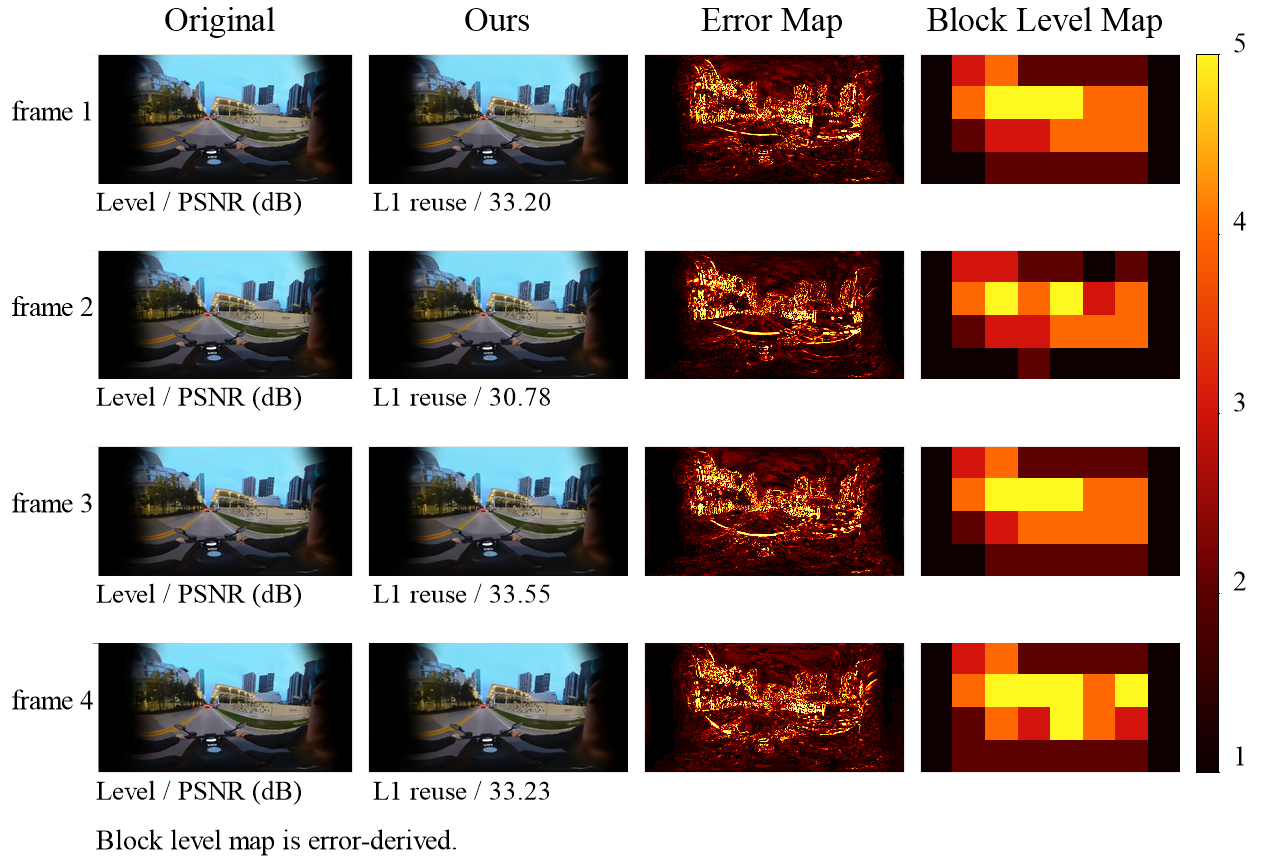
\includegraphics[width=0.8\textwidth]{qualitative_multiframe_vr.png}
\caption{Qualitative VR reconstruction examples with original frames, reconstructed frames, error maps, and block-level error maps.}
\label{fig:qualitative}
\end{figure*}

% --------------------------
% --------------------------
% --------------------------
% --------------------------

\section{Discussion}

The experiments lead to three conclusions. First, temporal redundancy remains useful after VAE encoding. LRC reduces payload because consecutive latent tensors are often close. Second, panoramic video benefits more from the proposed optimization than the 2D video because the tested VR sequence changes slowly and ERP geometry provides latitude-dependent redundancy. Third, the current system is weaker than mature codecs in classical rate-distortion performance. This negative result matters: semantic communication should not be evaluated only against its own internal baseline.

For wireless and mobile XR systems, the main implication is architectural. A conventional video file is usually treated as a byte stream whose internal dependencies are codec-specific. The semantic prototype exposes frame events with different network meanings. Level 1 reuse events are small but require timely control signalling. Full-latent updates refresh receiver state. Residual-latent updates may be smaller but depend on a valid previous latent. A future scheduler could prioritize full updates after scene changes, protect residual chains, or drop low-importance updates when latency budgets are exceeded.

\subsection{Toward a Network-Adaptive Semantic Stream}

A practical network-adaptive version would require several mechanisms beyond the current prototype. First, frame descriptors should identify whether an event is a reuse, full-latent, or residual-latent update, and should expose dependency information for residual chains. Second, the sender should estimate event importance. A full-latent update after a scene change should receive stronger protection than a reuse event during a static segment. Third, the transport layer should decide whether to retransmit, skip, or downgrade an update based on the remaining display deadline. Fourth, the receiver should report quality or state confidence, allowing the sender to insert refreshes when the cached latent becomes unreliable.

These mechanisms 
%are consistent with the MSWiM emphasis on modeling, analysis, and performance evaluation. They 
turn semantic video transmission into a system-level scheduling problem: the question is not only how many bytes are sent, but which visual state updates should be delivered before their deadlines.

% --------------------------
% --------------------------
% --------------------------
% --------------------------

\section{Limitations}

The present evaluation is intentionally limited. The frame-level loss model does not simulate packet-level wireless loss, packet reordering, congestion, or MAC-layer retransmission. The video set contains only two short clips. The AI components are pretrained and not optimized end-to-end for compression or channel robustness. The prototype also omits viewport prediction, head-motion traces, and subjective XR quality assessment. These limitations mean that the results should be read as a diagnostic evaluation of stream structure, not as evidence of deployable XR transport performance.

Another limitation is computational. The current paper reports visual payload and reconstruction quality, but it does not measure the full real-time processing chain: CLIP inference, VAE encoding, compression, transmission, decompression, VAE decoding, SwinIR restoration, and display synchronization. XR systems are latency-sensitive, so future evaluation must report end-to-end delay and energy consumption in addition to payload and PSNR.

Finally, the current semantic decision is global. CLIP similarity may not detect small but task-critical local changes. This is important for XR use cases such as remote assistance, where a small warning light or tool position can be more important than global scene similarity. Local object-aware or viewport-aware decision modules are therefore needed before the architecture can be used in safety-critical interactive applications.

% --------------------------
% --------------------------
% --------------------------
% --------------------------

\section{Conclusion}

This paper evaluated a semantic XR video transmission prototype under a frame-level update loss model. The system combines CLIP-based semantic reuse, VAE latent transmission, latent residual coding, latitude-adaptive quantization, and SwinIR restoration. LRC/LAQ reduces the prototype's own visual payload, especially on the panoramic sequence, but mature codecs remain far more efficient in rate-distortion terms and H.264 remains ahead under the tested loss model. The main contribution is therefore a network-oriented interpretation of semantic video streams: explicit reuse, full-update, and residual-update events create control points that future wireless XR transport protocols could schedule, protect, retransmit, or skip.

\section*{Acknowledgment}

This work was supported by the following projects: TRUE Wi-Fi PID2024-155470NB-I00 (MICIU/AEI/10,13039/501100011033/FEDER,UE), MLDR (Chist-ERA WAI 2022) PCI2023-145958-2 (MCIU/AEI/10.13039), ICREA Academia 2024 (00077 AGAUR), and MdM CEX2021-001195-M (MICIU/AEI/10.13039/501100011033).

\bibliographystyle{IEEEtran}
\bibliography{bibliography}

\end{document}
